\documentclass[11pt]{article}
\usepackage[a4paper,margin=2cm]{geometry}
\usepackage[utf8]{inputenc}
\usepackage{mathptmx} % times roman, including math
\usepackage[hyphens]{url}
\usepackage{doi}
\usepackage{hyperref}
\usepackage[numbers,sort]{natbib}
\usepackage{amsmath}
\usepackage{amssymb}
\usepackage{stmaryrd} % \llbracket etc.
\usepackage{setspace}
\usepackage{csquotes}
\usepackage{tikz}
\usetikzlibrary{arrows.meta}
\hyphenation{da-ta-cen-ter da-ta-cen-ters time-stamp time-stamps time-stamped Grish-chen-ko}
\frenchspacing

\usepackage{isabelle,isabellesym}
\isabellestyle{it}

\begin{document}
\sloppy
\title{OpSets: Concurrent Datatypes with Sequential Specifications}
%\title{OpSets: Sequential Specifications for Concurrent Editing}
\author{}
\date{}
\maketitle

\subsection*{Abstract}
TODO

\section{Introduction}

A common requirement across a great variety of systems is that several participants may concurrently access and manipulate some shared data structure.
However, unconstrained concurrent manipulation may introduce inconsistencies that applications cannot tolerate.
Thus, various approaches for providing \emph{consistency guarantees} have been developed, ensuring that the data structure continues to obey certain invariants or semantics under concurrent access. For example:

\begin{description}
\item[Transaction isolation] in databases restricts the degree to which concurrently executing transactions can affect each other while accessing the same database.
The strongest isolation level, \emph{serializability}, ensures that transactions behave as if there were no concurrency at all, i.e.\ as if transactions were executed serially, one at a time \cite{Kleppmann:2017wj}.

\item[Conflict-free Replicated Data Types (CRDTs)] allow each participant to modify a local copy (\emph{replica}) of a shared data structure without waiting for communication with other replicas \cite{Shapiro:2011wy,Shapiro:2011un}.
This has the consequence that the state of replicas may temporarily diverge, but the definition of CRDTs ensures that all replicas eventually converge towards a consistent state.

\item[Operational Transformation (OT)] algorithms are designed for several users who are concurrently editing a shared document \cite{Ellis:1989ue,Sun:1998un}, as implemented for example in Google Docs \cite{DayRichter:2010tt}.
As with CRDTs, OT allows each user's changes to be applied immediately to their local copy, while ensuring that other users' concurrent edits can be integrated in a consistent way.
\end{description}

We discuss these techniques in more detail in Section~\ref{sec:relwork}.
Despite decades of research in the above topics, consistency mechanisms for concurrent data access remain poorly understood, and tools for reasoning about them (both formally and informally) are subtle and error-prone.
As we show in the following sections, many published algorithms exhibit serious anomalies, or fail to even ensure convergence of replicas, leaving the system in a permanently inconsistent state \cite{Oster:2005vi,Imine:2003ks,Imine:2006kn}.

In this work we introduce \emph{Operation Sets} (or \emph{OpSets} for short), a novel approach for describing and reasoning about algorithms for concurrent data access and manipulation.
We go beyond merely ensuring replica convergence, and show how this approach simplifies the task of specifying and verifying stronger correctness properties.

Our contributions in this paper are as follows:

\begin{itemize}
\item We introduce the OpSet, a new abstraction for specifying and reasoning about the consistency properties of concurrently editable data structures.
On top of this abstraction, we specify a variety of abstract datatypes (maps, lists, trees, and registers), and we demonstrate that our specification is both simpler and more precise than previous efforts to specify the semantics of these data structures.

\item We demonstrate that our datatype specification captures an important correctness property that has been overlooked by prior work in this area.
Using our specification we review a selection of algorithms from the literature, and identify several that fail to satisfy this correctness property.

\item Using the Isabelle/HOL proof assistant, we formally verify the consistency of our semantics with alternative approaches, and prove that selected algorithms satisfy the semantics.
By using mechanised proofs we eliminate the ambiguity of previous informal approaches, and we can rule out reasoning errors that could occur in handwritten proofs.
\end{itemize}

% Uniform representation; easier to add new operation types

% Constrain operation: not allowed to have a return value. For example, CAS

\section{Background}\label{sec:background}

At a high level, consistency models for distributed data systems can be classified into two categories:
\begin{description}
\item[Strong consistency models] such as serialisability or linearisability \cite{Herlihy:1990jq} attempt to make a system behave like a single sequentially executing node, even when it is in fact replicated and concurrent.
An unavoidable downside of these models is that they require waiting for synchronous network communication before any operation or transaction is allowed to complete \cite{Davidson:1985hv,Gilbert:2002il}.
Thus, a node cannot make progress while it is offline or partitioned from other nodes.
In a formal sense, enforcing a strong consistency model is equivalent to consensus \cite{Chandra:1996cp,Herlihy:1991gk}, which implies that the algorithm cannot be guaranteed to terminate in an asynchronous system \cite{Fischer:1985tt}.

\item[Weak consistency models] are employed by systems that prioritise availability over strong consistency; for example, systems that require nodes to be able to make progress while offline or while partitioned from other nodes.
In such systems, each node typically reads and manipulates a local copy of the shared state, and propagates any changes to that state asynchronously to other nodes.
Examples of weak consistency models in this category are \emph{causal consistency} \cite{Attiya:2015dm,Mahajan:2011wz,Lloyd:2011hz} and \emph{eventual consistency} \cite{Bailis:2013jc,Burckhardt:2014hy,Terry:1994fp,Vogels:2009ca}.
\end{description}

In this work we focus on the latter category of weak consistency models.
However, as we shall demonstrate shortly, the OpSets approach allows us to specify our consistency model more precisely than existing techiques permit.

\subsection{Eventual Consistency is Insufficient}\label{sec:eventual-consistency}

Eventual consistency is usually informally defined as follows: \emph{if no new updates are made to the shared state, all nodes will eventually have the same data}.
This is a very weak definition for several reasons:
\begin{itemize}
\item The premise, \emph{if no new updates are made}, may never be true (if the shared state is continually modified because the system is never quiescent).
In that case, eventual consistency becomes a vacuous statement.

\item Many trivial algorithms satisfy the requirement of converging towards the same state.
For example, a system could simply discard writes, and thus converge to a state in which operations have been ignored.
Although such a system would not be useful in practice, the definition of eventual consistency does not capture the requirement that writes should be persistent.

\item In a system that allows nodes to make progress while they are partitioned from other nodes, it is inevitable that the local state of individual nodes might diverge due to concurrent modifications.
Such divergent states must then be merged at a later time, when communication between the nodes is restored.
Even if we require that this merge operation does not discard data that has been written, eventual consistency does not specify which states should be considered valid results of the merge operation.
We show in Section~\ref{sec:bad-merge} how such under-specification can lead to undesirable outcomes.
\end{itemize}

\subsection{Example: Merging Text Edits}\label{sec:bad-merge}

To demonstrate a problem with an under-specified consistency model, consider the example in Figure~\ref{fig:bad-merge}.
In this example, two users are concurrently editing a text document that initially reads ``Hello!''.
The user on the left changes it to read ``Hello Alice!'', while concurrently the user on the right changes the document to read ``Hello Charlie!''.
When the concurrent edits are merged, the algorithm randomly interleaves the two insertions of ``~Alice'' and ``~Charlie'' character by character, resulting in an unreadable jumble of characters.

\begin{figure}
\centering
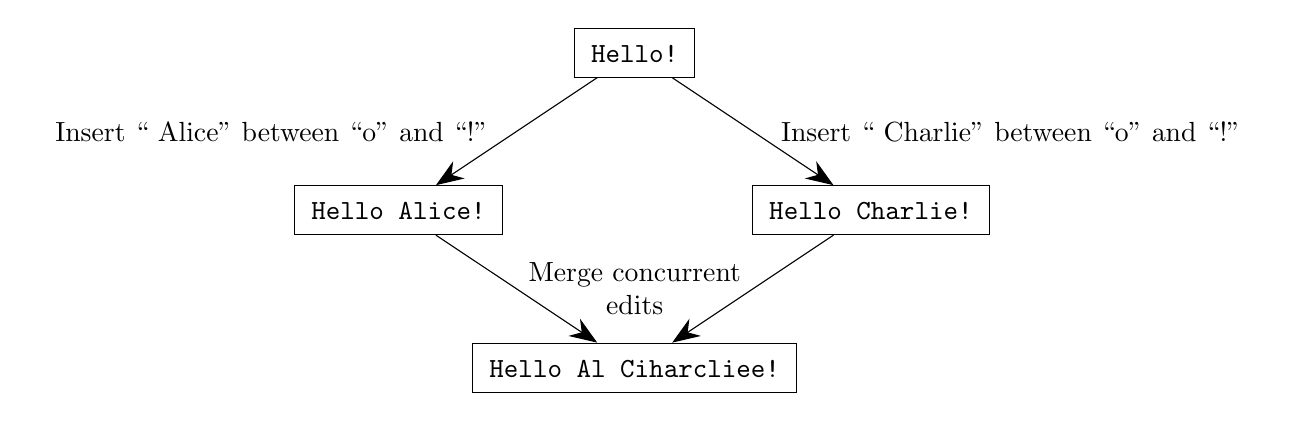
\begin{tikzpicture}
  \tikzstyle{box}=[rectangle,draw,inner xsep=6pt,text height=9pt,text depth=2pt]
  \tikzstyle{every path}=[draw,-{Stealth[length=3.5mm]}]
  \node [box] (start) at (3,4) {\texttt{Hello!}};
  \node [box] (left)  at (0,2) {\texttt{Hello Alice!}};
  \node [box] (right) at (6,2) {\texttt{Hello Charlie!}};
  \node [box] (merge) at (3,0) {\texttt{Hello Al Ciharcliee!}};
  \draw (start) to node [left,inner xsep=10pt]  {Insert ``~Alice'' between ``o'' and ``!''} (left);
  \draw (start) to node [right,inner xsep=10pt] {Insert ``~Charlie'' between ``o'' and ``!''} (right);
  \draw (left)  -- (merge);
  \draw (right) -- (merge);
  \node [text width=3cm,text badly centered] at (3,1) {Merge concurrent edits};
\end{tikzpicture}
\caption{Two concurrent insertions at the same position are interleaved.}\label{fig:bad-merge}
\end{figure}

The problem is even worse if the concurrent insertions are not just a single word, but an entire paragraph or section.
In these cases, interleaving the users' insertions would most likely result in an entirely incomprehensible text that would have to be deleted and rewritten.

Even though the merge in Figure~\ref{fig:bad-merge} is so obviously undesirable, there is to our knowledge no formal specification of collaborative text editing that rules out such an interleaving of insertions.
For example, the recent formal specification of collaborative text editing by Attiya et al.~\cite{Attiya:2016kh} allows the outcome in Figure~\ref{fig:bad-merge}.
Paraphrased informally, Attiya et al.'s specification requires that all character insertions and deletions take effect (no input is lost), and that the relative ordering of all characters is preserved (in the merged result, ``A'' comes before ``l'', which comes before ``i'', which comes before ``c'', etc).
An interleaved result, as in Figure~\ref{fig:bad-merge}, satisfies both of these requirements.

Moreover, several published algorithms for collaborative text editing allow the anomaly shown in Figure~\ref{fig:bad-merge}, and to our knowledge this anomaly has not been previously discussed in the literature.
We discuss these algorithms further in Section~\ref{sec:relwork}.

Rather than interleaving characters, a better approach to merging is to keep all insertions by a particular user together as a continuous sequence.
With this constraint, there are two acceptable merged results in the example of Figure~\ref{fig:bad-merge}: either ``Hello Alice Charlie!'' or ``Hello Charlie Alice!''.
The choice between these two outcomes is arbitrary, as there is no a priori requirement for one user's insertions to come before another's.
In Section~\ref{sec:datatypes} we give a specification that incorporates this constraint.

\section{The OpSets Approach}\label{sec:approach}

The OpSets approach is a simple abstraction for describing the consistency properties of a replicated data system.
We outline the general approach in this section, before describing concrete data structures and specifications in \S~\ref{sec:datatypes} and \S~\ref{sec:tree}.

\subsection{System Model}\label{sec:system-model}

We assume that the system consists of a set of \emph{nodes} connected by a \emph{network}.
These nodes concurrently access some \emph{shared data structure}, which may be a relational database (consisting of rows in tables), a text document (a sequence of characters), a vector-graphics document (a tree of records describing graphical objects), a filesystem (a tree of directories and files), or any other kind of data structure.

New nodes can be added at any time, and the set of nodes need not be known in advance.
Nodes might be mobile devices, and hence we assume that nodes are sometimes \emph{offline}, i.e.\ temporarily unable to communicate with other nodes.
We require that nodes can access the shared data anytime, even while offline.
Thus, each node has a local copy of the shared data structure, which it can read and modify without waiting for any communication or coordination with other nodes.

Whenever a node makes a modification to that structure, it records the change as an \emph{operation}.
For example, an operation may describe an insertion at a particular position in a text document.
Each node locally maintains a set of operations, the \emph{OpSet}.
Whenever a node makes a change to the shared data, it adds the corresponding operation to its OpSet, and also sends \emph{messages} containing the operation to other nodes.
Whenever a node receives a message from another node, the operation in that message is added to the recipient's local OpSet.
Operations remain immutable throughout this process.

We make no assumptions about the reliability of the network: messages may be lost, duplicated, or arbitrarily reordered.
Reflecting the characteristics of real networks, we assume that lost messages are retransmitted when possible (e.g.\ using TCP), but messages may be permanently lost due to network or node failures.
Since the OpSet at each node is a monotonically growing set of operations, any two communicating nodes can merge their OpSets using the standard set union operator $\cup$.
Set union is commutative, associative, and idempotent, ensuring that communicating nodes converge towards the same OpSet contents.

We assume that each operation has a unique identifier (ID), that new IDs can be generated by any node without communication with other nodes, and that we have a total ordering on operation IDs.
These requirements can easily be met by using Lamport timestamps \cite{Lamport:1978jq} as IDs.
A Lamport timestamp is a pair $(\mathit{counter}, \mathit{nodeID})$ that is constructed as follows:
\begin{itemize}
\item $\mathit{counter}$ is an integer.
    To generate a new ID, find the maximum counter of any existing operation ID in the local OpSet, and increment that number.
\item $\mathit{nodeID}$ is a string that uniquely identifies the node generating the ID, e.g.\ a UUID \cite{Leach:2005hm}.
\end{itemize}

Although different nodes may generate IDs with the same counter value, each node generates IDs with strictly increasing counter values, and thus IDs are globally unique.
We define the total order on IDs as being the lexicographic order:
\[
    \,(\mathit{ctr}_1, \mathit{node}_1) < (\mathit{ctr}_2, \mathit{node}_2)\,
    \;\Longleftrightarrow\;
    \mathit{ctr}_1 < \mathit{ctr}_2 \;\vee\;
    (\mathit{ctr}_1 = \mathit{ctr}_2 \wedge \mathit{node}_1 <\mathit{node}_2).
\]

%This total order is a linear extension of the partial order that captures their causal dependencies (the \emph{happens-before} relation).
%That is, whenever a node changes the shared data and generates a new operation, the ID of the new operation must be strictly greater than that of any existing operation in the OpSet of the node generating the new operation.

\subsection{Interpreting an OpSet}\label{sec:op-serial}

Most definitions of operation-based CRDTs describe how a node's local state is manipulated by operations \cite{Shapiro:2011wy,Shapiro:2011un}.
We now depart from this convention and present an alternative formulation of replicated datatypes.

In the OpSets approach, we require that the shared data structure is never manipulated directly.
Instead, we use an \emph{interpretation function} $\llbracket-\rrbracket$ that takes an OpSet $O$ and returns the current state $\llbracket O \rrbracket$ of the shared data structure described by the OpSet.
The interpretation function is \emph{pure}, i.e.\ deterministic, side-effect free, and its result depends only on $O$.
All nodes in the system employ the same interpretation function.

Consequently, whenever any two nodes have the same OpSet $O$, their view of the shared data structure $\llbracket O \rrbracket$ must also be equal.
This construction trivially ensures eventual consistency: as two nodes converge towards the same OpSet contents, any data structure that is deterministically derived from the OpSet must also converge.

In principle, any deterministic function can serve as interpretation function.
However, in defining the semantics of CRDTs (see \S~\ref{sec:datatypes} and \S~\ref{sec:tree}), we have found it useful to specialise $\llbracket-\rrbracket$ such that we can interpret one operation at a time.

Let the OpSet $O$ be a set of pairs $(\mathit{id},\, \mathit{op})$, where $\mathit{id}$ is a unique operation identifier and $\mathit{op}$ is an arbitrary description of the change that occurred.
Assume that we have a total ordering $<$ on identifiers, as explained in \S~\ref{sec:system-model}.
Then observe that for any OpSet there exists a unique sequence of operations, containing all operations of the OpSet in ascending order of their identifier.
We can specify the semantics of each operation~--- that is, the effect of the operation on the OpSet interpretation~--- when applied in this sequential order.

Formally, we can define the interpretation $\llbracket O \rrbracket$ of the OpSet $O$ as follows:
\begin{align*}
    \big\llbracket \emptyset \big\rrbracket &= \mathsf{InitialState} \\
    \big\llbracket O \;\cup\; \{(\mathit{id},\, \mathit{op})\} \big\rrbracket &=
    \mathsf{interp}\big[\llbracket O \rrbracket,\, (\mathit{id},\, \mathit{op})\big]
    \qquad\text{ provided that } \forall\,(\mathit{id}',\, \mathit{op}') \in O.\; \mathit{id}' < \mathit{id}
\end{align*}
where $\mathsf{interp}\big[S,\, (\mathit{id},\, \mathit{op})\big]$ is the interpretation of the operation $(\mathit{id},\, \mathit{op})$ in the state $S$, and $\mathsf{InitialState}$ is a fixed minimal element (e.g. the empty tree, or empty list) of the replicated type described.
In other words, if $S$ is the result of interpreting all operations with identifiers less than $\mathit{id}$, then
$\mathsf{interp}\big[S,\, (\mathit{id},\, \mathit{op})\big]$ is the interpretation of the OpSet to which $(\mathit{id},\, \mathit{op})$ has been added.
For example, if $\mathit{id}_1 < \mathit{id}_2 < \mathit{id}_3$, we have:
\begin{align*}
    \big\llbracket \{(\mathit{id}_1,\ \mathit{op}_1),\;
    &(\mathit{id}_2,\ \mathit{op}_2),\,
    (\mathit{id}_3,\ \mathit{op}_3)\} \big\rrbracket \;=\\
    &\mathsf{interp}\big[\mathsf{interp}\big[\mathsf{interp}\big[\mathsf{InitialState},\,
    (\mathit{id}_1,\ \mathit{op}_1)\big],\,
    (\mathit{id}_2,\ \mathit{op}_2)\big],\,
    (\mathit{id}_3,\ \mathit{op}_3)\big]
\end{align*}
Provided that the operation interpretation $\mathsf{interp}\big[S,\, (\mathit{id},\, \mathit{op})\big]$ is deterministic, the OpSet interpretation function $\llbracket-\rrbracket$ is also deterministic, due to the fact that the operation order in the OpSet is unique.

\subsection{Receiving Messages Out-of-order}\label{sec:order-change}

Many computing systems are based on the idea of putting operations in some total order, and executing them in that order.
For example, serializable transactions \cite{Kleppmann:2017wj} and state machine replication \cite{Schneider:1990vy} follow this approach.
However, it is important to understand that the OpSet interpretation of \S~\ref{sec:op-serial} relies on a weaker notion of ordering than most systems.

With serializable transactions and state machine replication, once a transaction/operation has been executed in some state, its results are expected to be durable.
Thus, before executing some transaction $T_i$, the system needs to ensure that there is no pending transaction with a lower ID than $T_i$ (which would need to be executed before $T_i$), since otherwise the subsequent arrival of a transaction with lower ID would invalidate the state in which $T_i$ was executed.
However, ensuring this precondition is expensive: as we show in \S~\ref{sec:op-sequences}, it requires communication with at least a quorum of nodes; if the IDs are Lamport timestamps, it even requires communication with every single node \cite{Lamport:1978jq}.
If too many nodes are offline, the system cannot execute any transactions.

By contrast, our system model of \S~\ref{sec:system-model} requires nodes to always be able to read and modify the shared data, even when all nodes are offline.
Moreover, we do not assume any ordering guarantees from the network.
Thus, whenever there is some operation $(\mathit{id}_1, \mathit{op}_1) \in O$ in the OpSet $O$ of some node, it is possible that the node will subsequently receive a message containing $(\mathit{id}_2, \mathit{op}_2)$, where $\mathit{id}_2 < \mathit{id}_1$; that is, the later-arriving operation needs to be applied before the existing operation $(\mathit{id}_1, \mathit{op}_1)$ in the OpSet interpretation $\llbracket O \rrbracket$.

In the OpSet model, such out-of-order delivery of operations is no problem: the order in which operations are received has no effect on the OpSet $O$, and since we assume the interpretation function to be pure and side-effect free, the interpretation $\llbracket O \rrbracket$ can always be recomputed whenever new operations are added to $O$.

The interpretation function is an \emph{executable specification} that defines the expected result of interpreting a set of operations.
Presenting replicated datatypes in this manner has two significant advantages:
\begin{enumerate*}
\item
Unlike typical definitions of CRDT algorithms \cite{Shapiro:2011wy,Shapiro:2011un}, it is not necessary for the interpretation function $\mathsf{interp}\big[S,\, (\mathit{id},\, \mathit{op})\big]$ to commute with respect to other operations: any pure function can be used.
This fact makes it much simpler to specify the interpretation of operations, as we shall see in \S~\ref{sec:datatypes} and \S~\ref{sec:tree}.
\item
We can guarantee the existence of an implementation of each described datatype: the specification itself.
This is in contrast to axiomatic specifications, which may not be implementable, and require additional work to demonstrate than an implementation exists which satisfies the axiomatic description.
\end{enumerate*}

For practical implementations of replicated datatypes, a naive OpSet interpretation may exhibit poor performance, since nodes must potentially apply the same subset of operations repeatedly.
More efficient (and, most likely, more complex) algorithms for CRDTs can therefore be developed and shown to satisfy the OpSet-based specification---we do this in \S~\ref{sec:bad-merge}.

However, we have developed a practical JavaScript CRDT implementation around the OpSet model,\footnote{\url{https://github.com/automerge/automerge}} and found it to have some advantages: for example, users can easily inspect the editing history of a document, since every past version of the document is the interpretation of a particular subset of operations.
Moreover, using OpSets provides a straightforward mechanism for recovering from network partitions and failures, as missing operations may be retransmitted and added to the OpSets of previously partitioned nodes.
The details of this implementation are beyond the scope of this paper.

\section{An Insert-Only List}\label{sec:list}

As a first concrete example of the approach outlined in Section~\ref{sec:approach}, we now show how to construct an ordered list data structure using an OpSet.
We initially consider a list that only supports insertion of list elements, and we extend the definition to support deletion in the following sections.

Let us assume that an OpSet may contain two types of operation:
$\mathrm{makeList}(\mathit{Oid})$ creates a new, empty list, and
$\mathrm{insertAfter}(\mathit{Oid}, \mathit{Previous})$ inserts a new list element.
The $\mathit{Oid}$ parameter of each constructor is the unique identifier of the operation.
The second parameter of insertAfter determines the insertion position: to insert at the head of a list, $\mathit{Previous}$ should equal the $\mathit{Oid}$ of the prior makeList operation that created the list; otherwise, $\mathit{Previous}$ is the $\mathit{Oid}$ of a prior insertAfter operation, and the new list element is placed after that existing list element.

In Section~\ref{sec:assign} we will show how to associate a value with every list element; for now, we will consider the list to be merely a sequence of operation IDs (oids).
An oid thus has a dual purpose: to identify an operation, but also to identify the list or list element created by that operation.

\subsection{Constructing a List from an OpSet}

We must now define a deterministic function that takes a set of makeList and insertAfter operations, and produces a corresponding list.
We do this by arranging the operations into a tree, and traversing the tree in a deterministic order.
The algorithm in this section is based on Attiya et al.'s timestamped insertion tree \cite{Attiya:2016kh}, which is similar to Grishchenko's causal tree \cite{Grishchenko:2014eh}.

\begin{figure}
\centering
\begin{minipage}{8cm}
\begin{align*}
\mathit{OpSet} = \{ &
    \mathrm{makeList}(0),\; \mathrm{insertAfter}(5, 0) \\ &
    \mathrm{insertAfter}(9, 5),\; \mathrm{insertAfter}(13, 0), \\&
    \mathrm{insertAfter}(14, 13),\; \mathrm{insertAfter}(15, 14), \\&
    \mathrm{insertAfter}(17, 14),\; \mathrm{insertAfter}(23, 14) \}
\end{align*}
\end{minipage}
\hspace{20pt}
\begin{minipage}{6cm}
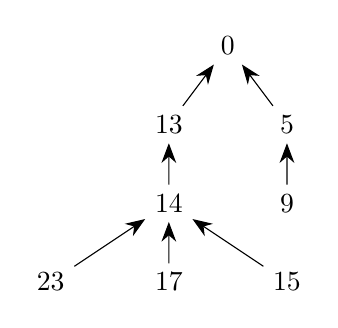
\begin{tikzpicture}[level distance=10mm]
  \tikzstyle{edge from parent}=[draw,{Stealth[length=2.5mm]}-]
  \node {0}
    child {node {13}
      child {node {14}
        child {node {23}}
        child {node {17}}
        child {node {15}}
      }
    }
    child {node {5}
      child {node {9}}
    };
\end{tikzpicture}
\end{minipage}
\caption{OpSet and corresponding tree representation of the list [13, 14, 23, 17, 15, 5, 9].}\label{fig:list-tree}
\end{figure}

Figure~\ref{fig:list-tree} shows an example of such an OpSet.
To construct the tree, we create a node for each operation, and make each insertAfter node a child of the node it references in its $\mathit{Previous}$ parameter.
A makeList operation forms the root of this tree.
The list order is determined by a depth-first pre-order traversal of this tree, ignoring the root node, and visiting any sibling nodes in order of descending oid.

\begin{figure}
\centering
\[ \mathit{nextElem} = \{ (0, 13),\; (13, 14),\; (14, 23),\; (23, 17),\; (17, 15),\; (15, 5),\; (5, 9) \} \]
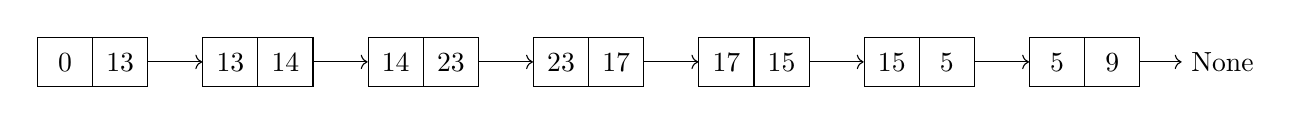
\begin{tikzpicture}
  \tikzstyle{every node}=[anchor=base,minimum width=7mm,text height=9pt,text depth=2pt]
  \matrix [column sep={7mm,between origins},nodes=draw] {
    \node (1a) {0};  & \node (1b) {13}; &&
    \node (2a) {13}; & \node (2b) {14}; &&
    \node (3a) {14}; & \node (3b) {23}; &&
    \node (4a) {23}; & \node (4b) {17}; &&
    \node (5a) {17}; & \node (5b) {15}; &&
    \node (6a) {15}; & \node (6b) {5};  &&
    \node (7a) {5};  & \node (7b) {9};  && \node (8a) [draw=none] {None}; \\
  };
  \draw [->] (1b) -- (2a);
  \draw [->] (2b) -- (3a);
  \draw [->] (3b) -- (4a);
  \draw [->] (4b) -- (5a);
  \draw [->] (5b) -- (6a);
  \draw [->] (6b) -- (7a);
  \draw [->] (7b) -- (8a);
\end{tikzpicture}
\vskip 12pt
After adding insertAfter(25, 13) to $\mathit{OpSet}$:
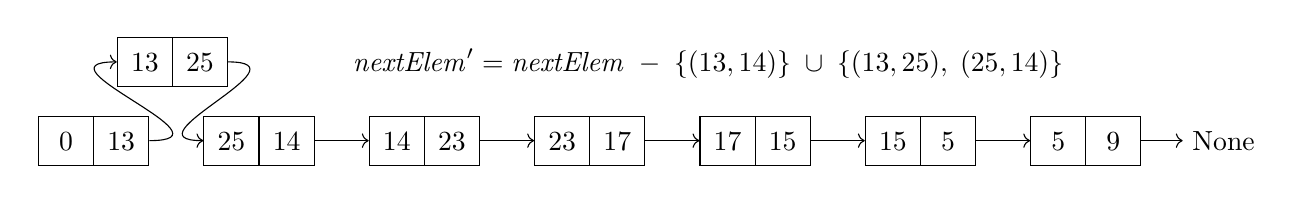
\begin{tikzpicture}
  \tikzstyle{every node}=[anchor=base,minimum width=7mm,text height=9pt,text depth=2pt]
  \node [anchor=west] at (4,1) {$\mathit{nextElem}' = \mathit{nextElem} \;-\; \{(13, 14)\} \;\cup\; \{(13, 25),\; (25, 14)\}$};
  \matrix [column sep={7mm,between origins},nodes=draw,matrix anchor=west] at (1,1) {
    \node (n1) {13}; & \node (n2) {25}; \\
  };
  \matrix [column sep={7mm,between origins},nodes=draw,matrix anchor=west] at (0,0) {
    \node (1a) {0};  & \node (1b) {13}; &&
    \node (2a) {25}; & \node (2b) {14}; &&
    \node (3a) {14}; & \node (3b) {23}; &&
    \node (4a) {23}; & \node (4b) {17}; &&
    \node (5a) {17}; & \node (5b) {15}; &&
    \node (6a) {15}; & \node (6b) {5};  &&
    \node (7a) {5};  & \node (7b) {9};  && \node (8a) [draw=none] {None}; \\
  };
  \draw [->] (1b.east) .. controls (2.7,0) and (0,1) .. (n1.west);
  \draw [->] (n2.east) .. controls (3.6,1) and (1.2,0) .. (2a.west);
  \draw [->] (2b) -- (3a);
  \draw [->] (3b) -- (4a);
  \draw [->] (4b) -- (5a);
  \draw [->] (5b) -- (6a);
  \draw [->] (6b) -- (7a);
  \draw [->] (7b) -- (8a);
\end{tikzpicture}
\caption{The nextElem relation derived from the OpSet in Figure~\ref{fig:list-tree}. It describes the order of list elements similarly to a linked list.}\label{fig:next-elem}
\end{figure}

\begin{figure*}
\begin{align*}
\mathrm{isListElem}(\mathit{Oid}) \leftarrow\; &
    \mathrm{insertAfter}(\mathit{Oid}, \mathit{Parent}).\\
\mathrm{hasChild}(\mathit{Parent}) \leftarrow\; &
    \mathrm{insertAfter}(\mathit{Child}, \mathit{Parent}).\\
\mathrm{laterChild}(\mathit{Parent}, \mathit{Child2}) \leftarrow\; &
    \mathrm{insertAfter}(\mathit{Child1}, \mathit{Parent}),\;
    \mathrm{insertAfter}(\mathit{Child2}, \mathit{Parent}),\;
    \mathit{Child1} > \mathit{Child2}.\\
\mathrm{firstChild}(\mathit{Parent}, \mathit{Child}) \leftarrow\; &
    \mathrm{insertAfter}(\mathit{Child}, \mathit{Parent}),\;
    \neg\;\mathrm{laterChild}(\mathit{Parent}, \mathit{Child}).\\
\mathrm{sibling}(\mathit{Child1}, \mathit{Child2}) \leftarrow\; &
    \mathrm{insertAfter}(\mathit{Child1}, \mathit{Parent}),\;
    \mathrm{insertAfter}(\mathit{Child2}, \mathit{Parent}).\\
\mathrm{laterSibling}(\mathit{Sib1}, \mathit{Sib2}) \leftarrow\; &
    \mathrm{sibling}(\mathit{Sib1}, \mathit{Sib2}),\;
    \mathit{Sib1} > \mathit{Sib2}.\\
\mathrm{laterSibling2}(\mathit{Sib1}, \mathit{Sib3}) \leftarrow\; &
    \mathrm{sibling}(\mathit{Sib1}, \mathit{Sib2}),\;
    \mathrm{sibling}(\mathit{Sib1}, \mathit{Sib3}),\;
    \mathit{Sib1} > \mathit{Sib2},\;
    \mathit{Sib2} > \mathit{Sib3}.\\
\mathrm{nextSibling}(\mathit{Sib1}, \mathit{Sib2}) \leftarrow\; &
    \mathrm{laterSibling}(\mathit{Sib1}, \mathit{Sib2}),\;
    \neg\;\mathrm{laterSibling2}(\mathit{Sib1}, \mathit{Sib2}).\\
\mathrm{hasNextSibling}(\mathit{Sib1}) \leftarrow\; &
    \mathrm{laterSibling}(\mathit{Sib1}, \mathit{Sib2}).\\
\mathrm{nextSiblingAnc}(\mathit{Start}, \mathit{Next}) \leftarrow\; &
    \mathrm{nextSibling}(\mathit{Start}, \mathit{Next}).\\
\mathrm{nextSiblingAnc}(\mathit{Start}, \mathit{Next}) \leftarrow\; &
    \neg\;\mathrm{hasNextSibling}(\mathit{Start}),\;
    \mathrm{insertAfter}(\mathit{Start}, \mathit{Parent}),\;
    \mathrm{nextSiblingAnc}(\mathit{Parent}, \mathit{Next}).\\
\mathrm{hasSiblingAnc}(\mathit{Start}) \leftarrow\; &
    \mathrm{nextSiblingAnc}(\mathit{Start}, \mathit{Next}).\\
\mathrm{nextElem}(\mathit{Prev}, \mathit{Next}) \leftarrow\; &
    \mathrm{firstChild}(\mathit{Prev}, \mathit{Next}).\\
\mathrm{nextElem}(\mathit{Prev}, \mathit{Next}) \leftarrow\; &
    \mathrm{isListElem}(\mathit{Prev}),\;
    \neg\;\mathrm{hasChild}(\mathit{Prev}),\;
    \mathrm{nextSiblingAnc}(\mathit{Prev}, \mathit{Next}).\\

\end{align*}
\caption{Datalog rules for an ordered list (insertion only).}\label{fig:list-insert-datalog}
\end{figure*}

More formally, 

Figure~\ref{fig:list-insert-datalog} gives a Datalog query that expresses this traversal.
For readers who are unfamiliar with Datalog, it can informally be read as follows: if all predicates on the right-hand side of an arrow can be satisfied by some variable assignment, then we can conclude that the left-hand side is also true.
Later rules build upon earlier rules to create more complex constructions.

\section{Maps, Trees, and Assignment}\label{sec:assign}


\section{Related Work}\label{sec:relwork}

Algorithms for collaboratively editing a shared data structure have been the topic of active research for approximately 30 years, under the headings of Operational Transformation \cite{Ellis:1989ue,Nichols:1995fd,Ressel:1996wx,Sun:1998un,Sun:1998vf,Suleiman:1997gl,Suleiman:1998eu,Vidot:2000ch,Imine:2003ks,Li:2004er,Li:2008hw,Oster:2006tr} and CRDTs \cite{Shapiro:2011wy,Shapiro:2011un,Roh:2011dw,Preguica:2009fz,Oster:2006wj,Weiss:2010hx,Nedelec:2013ky,Nedelec:2016eo,Grishchenko:2014eh,Kleppmann:2016ve}.

However, throughout this time, the exact consistency properties provided by the algorithms have been somewhat unclear.
For example, Sun et al.~\cite{Sun:1998un} identified three desirable properties that they articulated informally: \emph{convergence}, \emph{causality preservation}, and \emph{intention preservation}.
While the definition of the first two properties is fairly unambiguous, the definition of ``intention preservation'' leaves much more room for interpretation.
Sun et al.\ define it as follows \cite{Sun:1998un}:
\begin{displayquote}
For any operation $O$, the effects of executing $O$ at all sites are the same as the intention of $O$, and the effect of executing $O$ does not change the effects of independent operations.
\end{displayquote}
where the term \emph{intention} is in turn defined as:
\begin{displayquote}
The intention of an operation $O$ is the execution effect which can be achieved by applying $O$ on the document state from which $O$ was generated.
\end{displayquote}
Efforts to formally specify and verify the semantics of replicated datatypes have replaced informal statements of this type with more precise definitions of consistency properties.

\subsection{Specification and Verification}

Bieniusa et al.~\cite{Bieniusa:2012gt} articulate a \emph{principle of permutation equivalence} that partially specifies the expected semantics of replicated datatypes, but which leaves some combinations of operations unspecified.
Burckhardt et al.~\cite{Burckhardt:2014ft} give a complete specification of CRDT counters, registers, and sets, and show how to verify that algorithms satisfy these specifications in hand-written proofs.
Zeller et al.~\cite{Zeller:2014fl} formalise the same datatypes using Isabelle/HOL and provide mechanised proofs of their correctness.
These papers do not consider lists, maps, or tree datatypes.

Gomes et al.~\cite{Gomes:2017gy} establish a formal verification framework for CRDTs in Isabelle/HOL, and verify the strong eventual consistency properties (in particular, convergence) of a list, set, and counter datatype.
However, the work does not specify the datatype semantics beyond the convergence property.

Attiya et al.~\cite{Attiya:2016kh} give two specifications of collaborative text editing ($\mathcal{A}_\textsf{strong}$ and $\mathcal{A}_\textsf{weak}$), prove that the RGA CRDT \cite{Roh:2011dw} satisfies $\mathcal{A}_\textsf{strong}$, and conjecture that the Operational Transformation algorithm Jupiter \cite{Nichols:1995fd} satisfies $\mathcal{A}_\textsf{weak}$.
Wei et al.~\cite{Wei:2017tg} complete the proof that Jupiter satisfies $\mathcal{A}_\textsf{weak}$.

XXX: also~\cite{DBLP:conf/popl/BurckhardtGYZ14, DBLP:conf/atva/MukundRS15, DBLP:conf/coordination/GadducciMR17, DBLP:conf/popl/GotsmanYFNS16}

\subsection{Collaborative Tree Datatypes}

For collaborative editing of tree data structures, several CRDTs \cite{Martin:2010ih,Kleppmann:2016ve} and Operational Transformation algorithms \cite{Jungnickel:2016cb,Ignat:2003jy,Davis:2002iv} have been proposed.
However, most of them only consider insertion and deletion of tree nodes, but do not support a move operation.

As explained in Section~\ref{sec:tree}, supporting an operation that can move a subtree to a new location within a tree raises the possibility of some particular conflicts that need to be handled.
Ahmed-Nacer et al.~\cite{AhmedNacer:2012us} survey approaches to handling these conflicts without providing concrete algorithms.
Tao et al.~\cite{Tao:2015gd} propose handling conflicting move operations by allowing the same object to appear in more than one location; thus, their datatype is strictly a DAG, not a tree.

Najafzadeh~\cite{Najafzadeh:2017vk} asserts that concurrent move operations on a tree cannot safely be implemented in a CRDT, since the precondition of a move operation is not stable.
The proposed solution in this work is to use locks to globally synchronise move operations, thus preventing a scenario such as that in Figure~\ref{fig:concurrent-move} from ever occurring.
However, the resulting datatype is not strictly a CRDT, since some operations require strongly consistent synchronisation.

To our knowledge, our move semantics specified in Section~\ref{sec:tree} is the first definition of such an operation on a fully asynchronous tree CRDT.
We avoid the apparent contradiction with Najafzadeh's assertion by evaluating the precondition $(\mathit{val},\, \mathit{obj}) \notin \mathrm{ancestor}(E)$ at the same time as applying the operation, rather than at the time when the operation is generated, and by applying all operations in the OpSet in a deterministic order.

\subsection{Ordered Sets of Operations}

Baquero et al.~\cite{Baquero:2014ed} and Grishchenko~\cite{Grishchenko:2014eh} have previously proposed representing CRDTs in terms of a partially-ordered log of operations (where the partial order captures the causal relationships between operations).
Our OpSet is a straightforward variant of this idea, in which we define the total order on identifiers to be a linear extension of the partial order that captures causality.
This linear extension is well-known and goes back to Lamport~\cite{Lamport:1978jq}.

Our approach of sequentially interpreting operations, in order of $\mathit{id}$, is reminiscent of the concept of \emph{serializability} in databases: the data structure obtained by interpreting an OpSet is equal to the outcome of applying the operations in their serial order, even if the execution that produced the OpSet was in fact concurrent.
However, conventional transaction serializability requires synchronous coordination between replicas \cite{Davidson:1985hv}.
We circumvent this limitation, and hence allow nodes to make progress while offline, by allowing the interpretation of an operation to change if another operation with a lower ID is delivered.


\bibliographystyle{plainnat}
\bibliography{references}{}
\end{document}
